\documentclass{beamer}
\usepackage[T1]{fontenc}
\usepackage{multicol}
\usepackage{ragged2e}   %new code
\usepackage[utf8]{inputenc}
\usepackage[brazil]{varioref}
\usepackage[square,sort,comma,super,authoryear]{natbib}
\usepackage{xmpmulti}
\usepackage{epsfig}
\usepackage{subcaption}
\captionsetup{compatibility=false}
\usepackage{ru,graphicx,hyperref,url} % 

\addtobeamertemplate{block begin}{}{\justifying}
\setbeamertemplate{section in toc}[sections numbered]
\AtBeginSection[]
{
  \begin{frame}{Table of Contents}
  \begin{multicols}{2}
      \tableofcontents[currentsection]
    \end{multicols}
  \end{frame}

}

% The title of the presentation:
%  - first a short version which is visible at the bottom of each slide;
%  - second the full title shown on the title slide;

\title[Modelling Cultural Heritage with Photography]{
 Modelling Cultural Heritage with Photography: a New Approach for Image Acquisition using UAV}

% Optional: a subtitle to be dispalyed on the title slide
% \subtitle{Show where you're from}

% The author(s) of the presentation:
%  - again first a short version to be displayed at the bottom;
%  - next the full list of authors, which may include contact information;
\author[Pedro Victor Vieira de Paiva]{
  Pedro Victor Vieira de Paiva\\
  Marco Antônio Garcia de Carvalho\\
  Eloisa Dezen-Kempter\\\medskip
  {\small {pedro.paiva@pos.ft.unicamp.br}
  }}

% The institute:
%  - to start the name of the university as displayed on the top of each slide
%    this can be adjusted such that you can also create a Dutch version
%  - next the institute information as displayed on the title slide
\institute[Universidade Estadual de Campinas ]{
  Laboratório de Computação Visual -- IMAGELab \\
  }

% Add a date and possibly the name of the event to the slides
%  - again first a short version to be shown at the bottom of each slide
%  - second the full date and event name for the title slide
\date{\today}

\begin{document}

\begin{frame}
  \titlepage
\end{frame}

\begin{frame}{Table of Contents}
    \begin{multicols}{2}
    \tableofcontents
    \end{multicols}
\end{frame}

% Section titles are shown in at the top of the slides with the current section 
% highlighted. Note that the number of sections determines the size of the top 
% bar, and hence the university name and logo. If you do not add any sections 
% they will not be visible.
\section{Motivation}
\subsection{Digital Documentation}
\begin{frame}
    \frametitle{Motivation}
    \framesubtitle{Digital Documentation}
    \justifying The current conditions of a construction, also called “as-is” building, must be correctly observed, obtained and analyzed in many applications \citep{remondino2011} such: 
    
    \begin{itemize}[<+-| alert@+>]
        \item Historic Documentation
        \item Restoration
        \item Conservation
    \end{itemize}
\end{frame}

\begin{frame}
    \frametitle{Motivation}
    \framesubtitle{Digital Documentation}
    \justifying Laser sensors are commonly applied in building data acquisition, resulting in an extremely precise representation, although expensive and its high computational cost.
    
    \begin{figure}
        \centering
        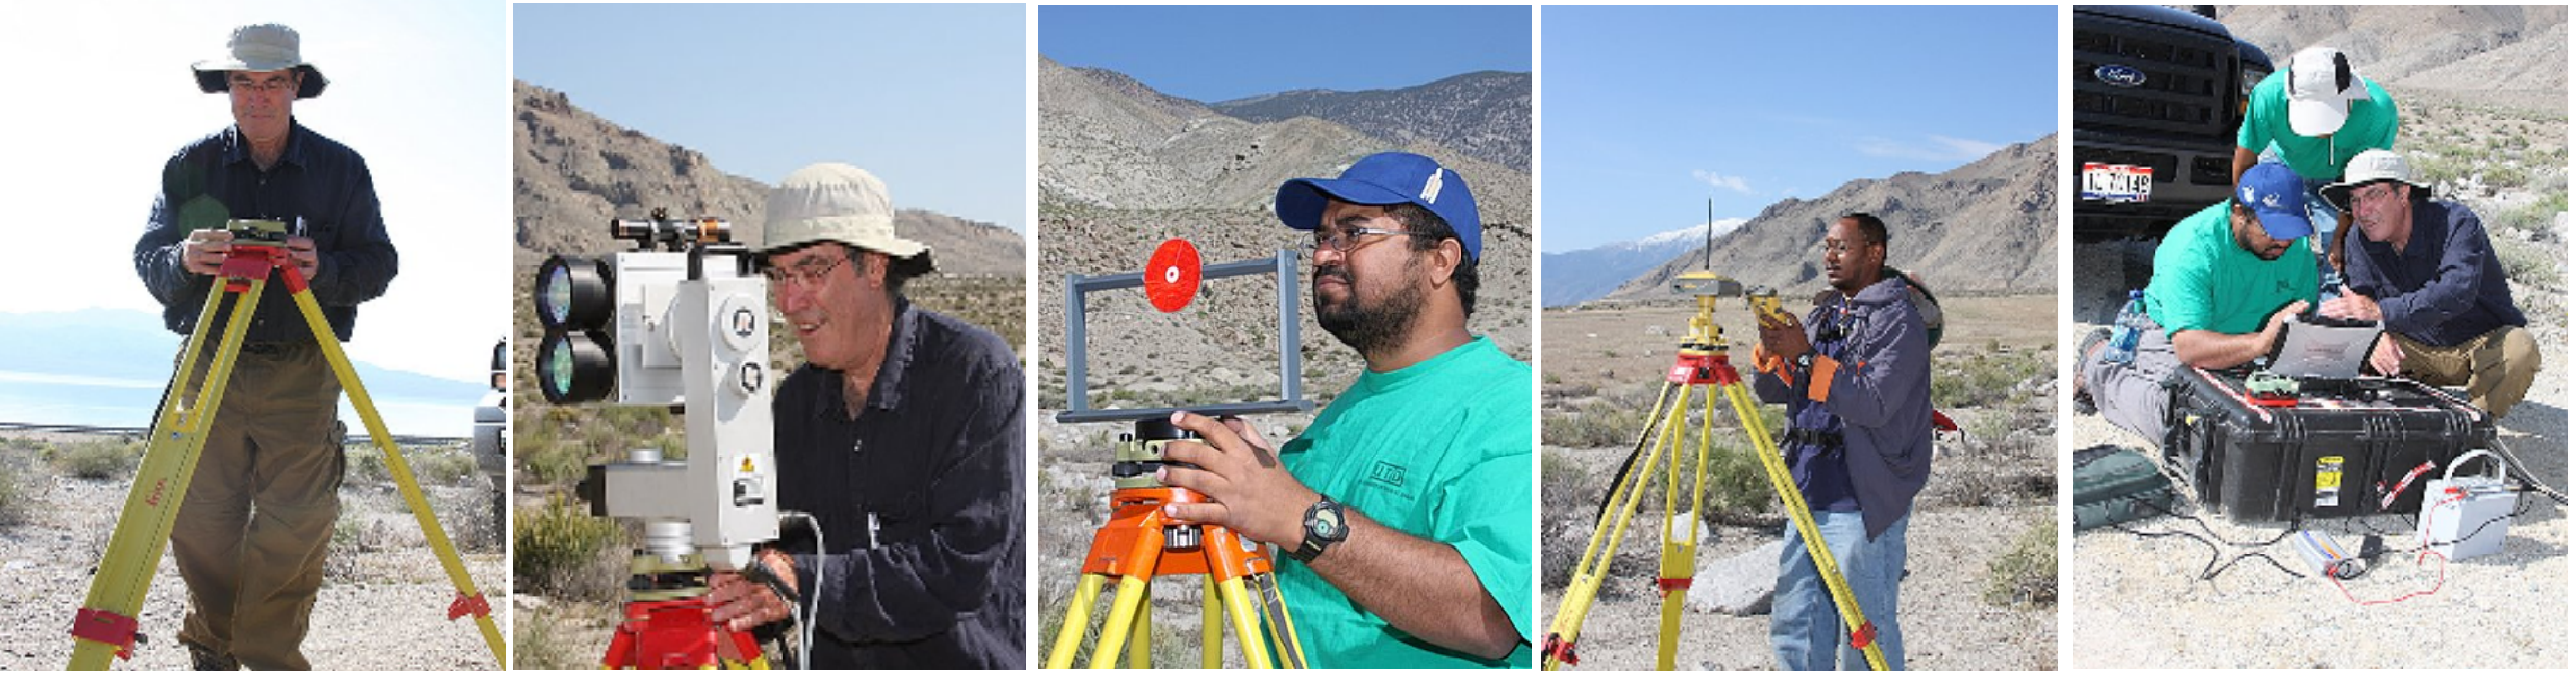
\includegraphics[scale=.16]{images/6}
        \caption{Field equipment necessary for acquisition. Source: \citep{oldow2008application}}
    \end{figure}
    
\end{frame}

\begin{frame}
    \frametitle{Motivation}
    \framesubtitle{Digital Documentation}

    \begin{block}{Point Cloud}
        \begin{figure}
        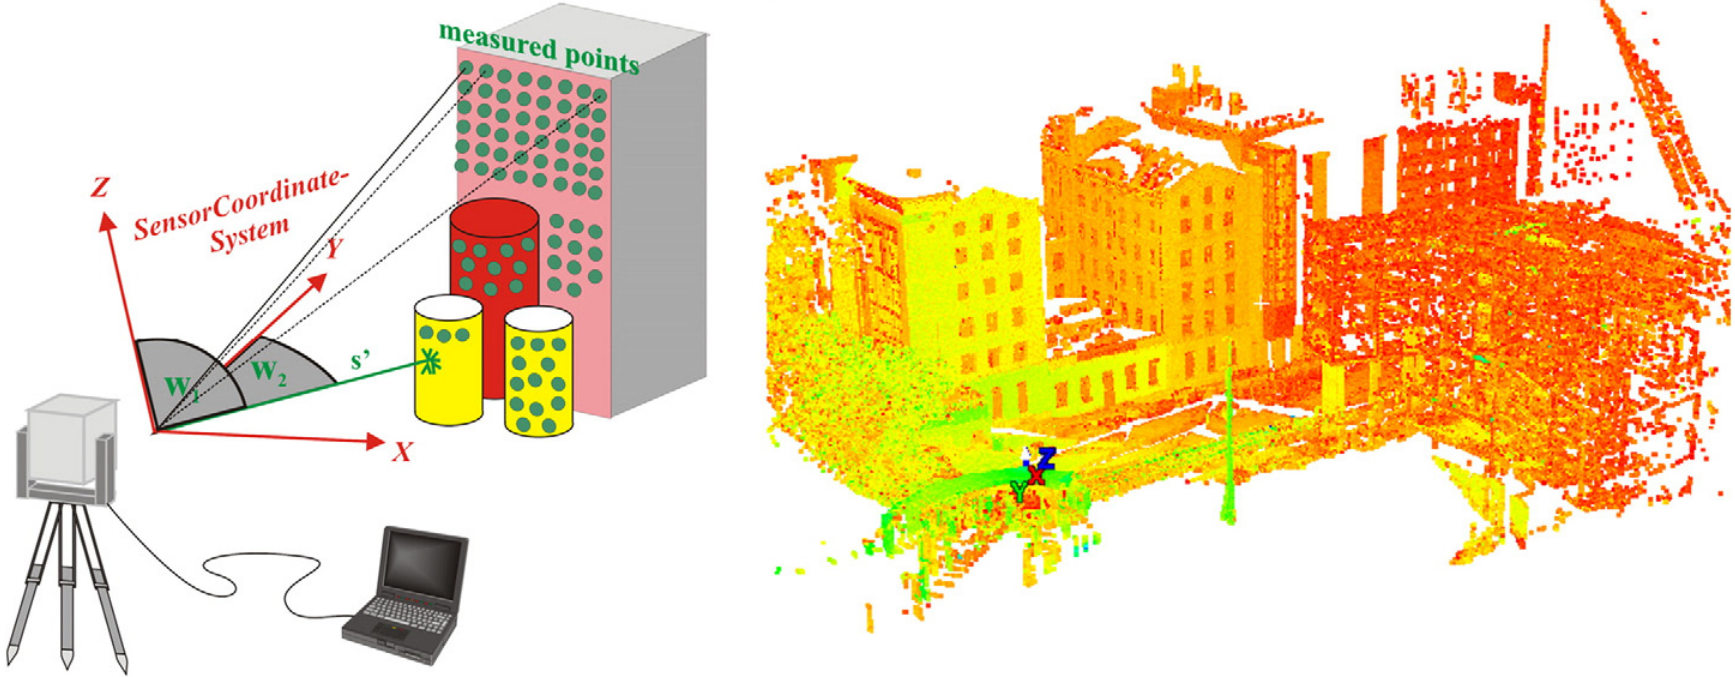
\includegraphics[scale=.2]{images/pc}
        \caption{The laser scanning process for measuring 3D point. Source: \citep{tang2010automatic}}
        \end{figure}
    \end{block}    
\end{frame}

\begin{frame}
    \frametitle{Motivation}
    \framesubtitle{Digital Documentation}
    \justifying
    Combining a large set of pictures, toke from different angle, and applying a method called \textit{Structure from Motion} a similar result can be achieved.

    \begin{figure}
        \centering
        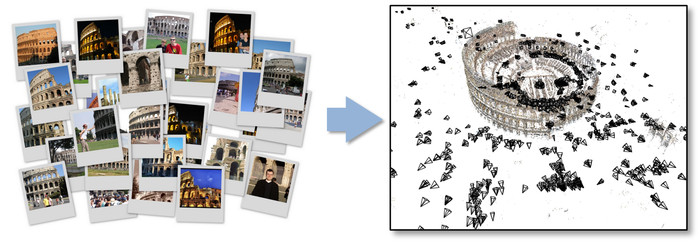
\includegraphics[scale=.7]{images/Colosseum}
        \caption{Point cloud generation with SfM. Source: Bundler Project.}
    \end{figure}
\end{frame}

\subsection{UAV acquisition difficulties}
\begin{frame}
    \frametitle{Motivation}
    \framesubtitle{UAV acquisition difficulties}
    \justifying 
    Unlike laser sensors, \textit{Unmanned Aerial Veichels} (UAV) with digital cameras are now affordable and user-friendly.
    \begin{figure}
        \centering
        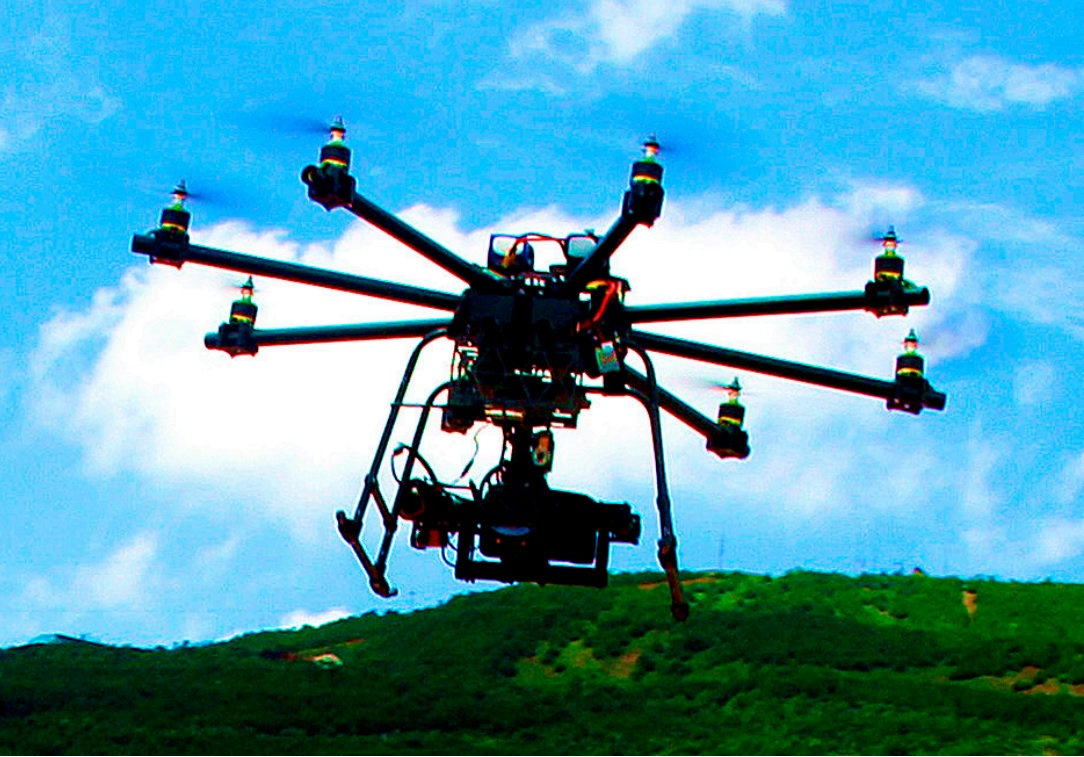
\includegraphics[scale=.18]{images/drone}
        \caption{Eight-rotor UAV platform (BNU-D8-1) fitted with Cannon 5DII. Source: \citep{xu2014tridimensional}.}
    \end{figure}
\end{frame}

\begin{frame}
    \frametitle{Motivation}
    \framesubtitle{UAV acquisition difficulties}
    \justifying Despite this, a universal data (image) acquisition protocol is not yet available, what make it an effective but still experimental process. Particularly in cultural heritage, is not a trivial task due:
    
    \begin{itemize}[<+-| alert@+>]
        \item Partial occlusion
        \item Element uniqueness
        \item Weather conditions
        \item etc...
    \end{itemize}
\end{frame}

\begin{frame}
    \frametitle{Motivation}
    \framesubtitle{UAV acquisition difficulties}
    \justifying 
    
    \begin{block}{Question}
   What is required to develop a standard protocol applicable to image acquisition of heritage by adopting UAV systems?
    \end{block}    
    
\end{frame}

\section{Theoretical Background}
\subsection{Photogrammetry}
\begin{frame}
  \frametitle{Theoretical Background}
  \framesubtitle{Photogrammetry}
  \justifying
   Photogrammetry is the science of making measurements from photographs, based on camera calibration.  
   
   \begin{figure}
        \centering
        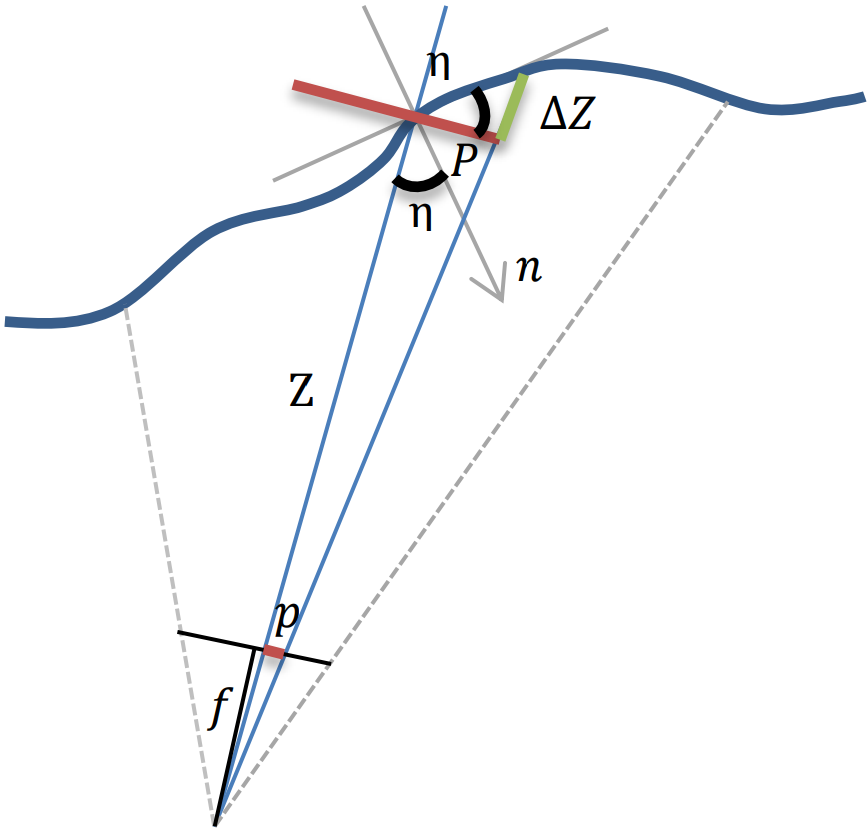
\includegraphics[scale=.15]{images/cam_par}
        \caption{Camera parameters for distance estimation. Source: \citep{wenzel2013image}}
    \end{figure}

\end{frame}

\begin{frame}
  \frametitle{Theoretical Background}
  \framesubtitle{Photogrammetry}
  \justifying
  According to \citep{murtiyoso2016acquisition}, there are different established and trustworthy image acquisition protocols. This methods share common characteristics, such as:
   
   \begin{itemize}
       \item Position and sensor calibration steps
       \item Angle convergence
       \item Image overlay
   \end{itemize}

\end{frame}

\subsection{Structure from Motion}
\begin{frame}
  \frametitle{Theoretical Background}
  \framesubtitle{Structure from Motion}
  \justifying
  
  \textit{Structure from Motion} (SfM) techniques uses overlapping pictures to extract object information by using camera internal parameters for orientation \citep{micheletti2015structure}.
 
    \begin{figure}
        \centering
        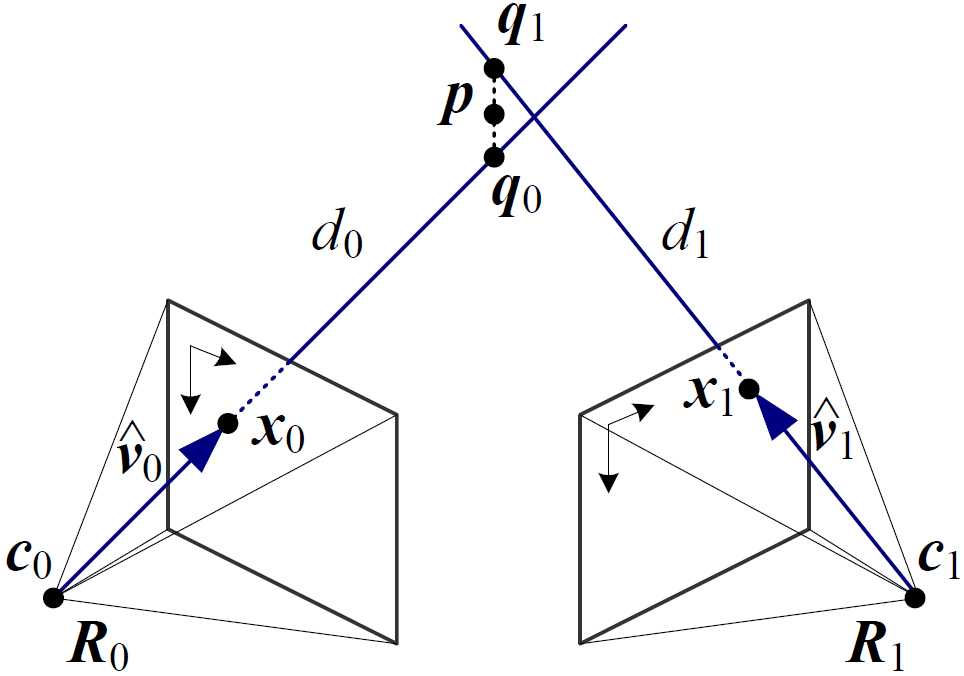
\includegraphics[scale=.17]{images/sfm}
        \caption{3D point triangulation by finding the point $\mathbf{p}$ that lies nearest to all of the optical rays $\mathbf{c}_{j} + d_{j}\mathbf{\hat{v}}_{j} $. Source: \citep{szeliski2010computer}}
    \end{figure}
\end{frame}


\begin{frame}
  \frametitle{Theoretical Background}
  \framesubtitle{Structure from Motion}
  \justifying
   For outstanding outcome, it is imperative:
   
   \begin{itemize}
       \item Generous collection of images
       \item Similar pictures took from rotated points of view (vertical and horizontal)
       \item Depth and range variable points of view
   \end{itemize}
  
\end{frame}


\section{Proposed Approach}
\begin{frame}{Proposed Approach}

\begin{block}{Pipeline}
        \begin{figure}
        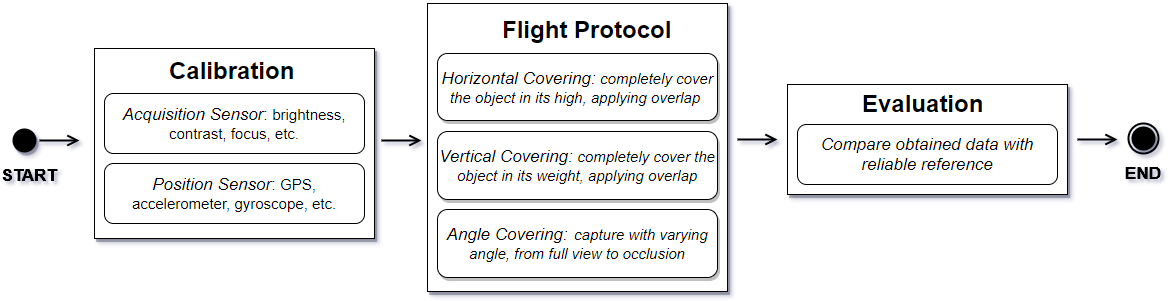
\includegraphics[scale=.35]{images/dia}
        \caption{Activity diagram of an effective approach for acquisition systems to structure modeling using SfM techniques. Source: author.}
        \end{figure}
    \end{block}    

\end{frame}

\subsection{Calibration}
\begin{frame}{Proposed Approach}
\framesubtitle{Calibration}
\justifying

\begin{itemize}
    \item 3D model construction requires precise sensor position estimation
    \begin{itemize}
        \item  Start from the highest point, allowing satellite synchronization (as much as possible).
    \end{itemize}
        \item Regarding the camera 
    \begin{itemize}
        \item Brightness, focus, contrast and saturation are currently well adjustable in auto-mode
    \end{itemize}
\end{itemize}
    
\end{frame}

\subsection{Flight Protocol}
\begin{frame}
  \frametitle{Proposed Approach}
  \framesubtitle{Flight Protocol}
  \justifying
  
  A path capable to cover full angle variation of the structure, parallel and perpendicular, is the hardest challenge in UAV flight planning.
  
  \begin{figure}[ht]
        \begin{minipage}[b]{0.45\linewidth}
            \justifying
            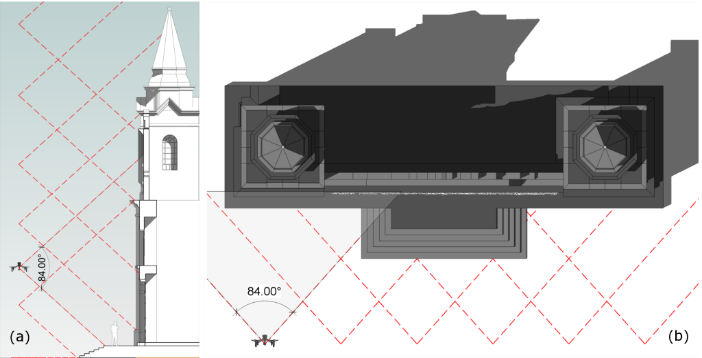
\includegraphics[width=\textwidth]{images/fpa}
            \caption{Height and weight portions fully covered.}
            \label{fig:a}
        \end{minipage}
        \hspace{0.5cm}
        \begin{minipage}[b]{0.45\linewidth}
             \justifying
            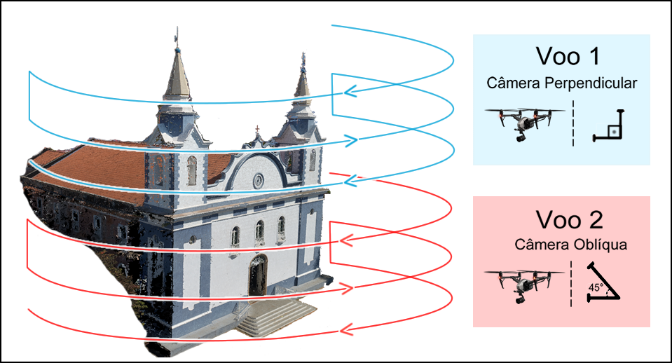
\includegraphics[width=\textwidth]{images/fpb}
            \caption{Flight plan with high angle variation.}
            \label{fig:b}
        \end{minipage}
    \end{figure}
    \vspace{-.5cm}
    \centering \small{(Source: author)}
\end{frame}

\subsection{Evaluation}

\begin{frame}{Proposed Approach}
  \framesubtitle{Evaluation}

    Once collected and processed, data could be evaluated comparing regional projection of point cloud to it equivalent “as-design”.    
    
    \begin{figure}
    \begin{subfigure}{1\linewidth}
        \begin{center}
            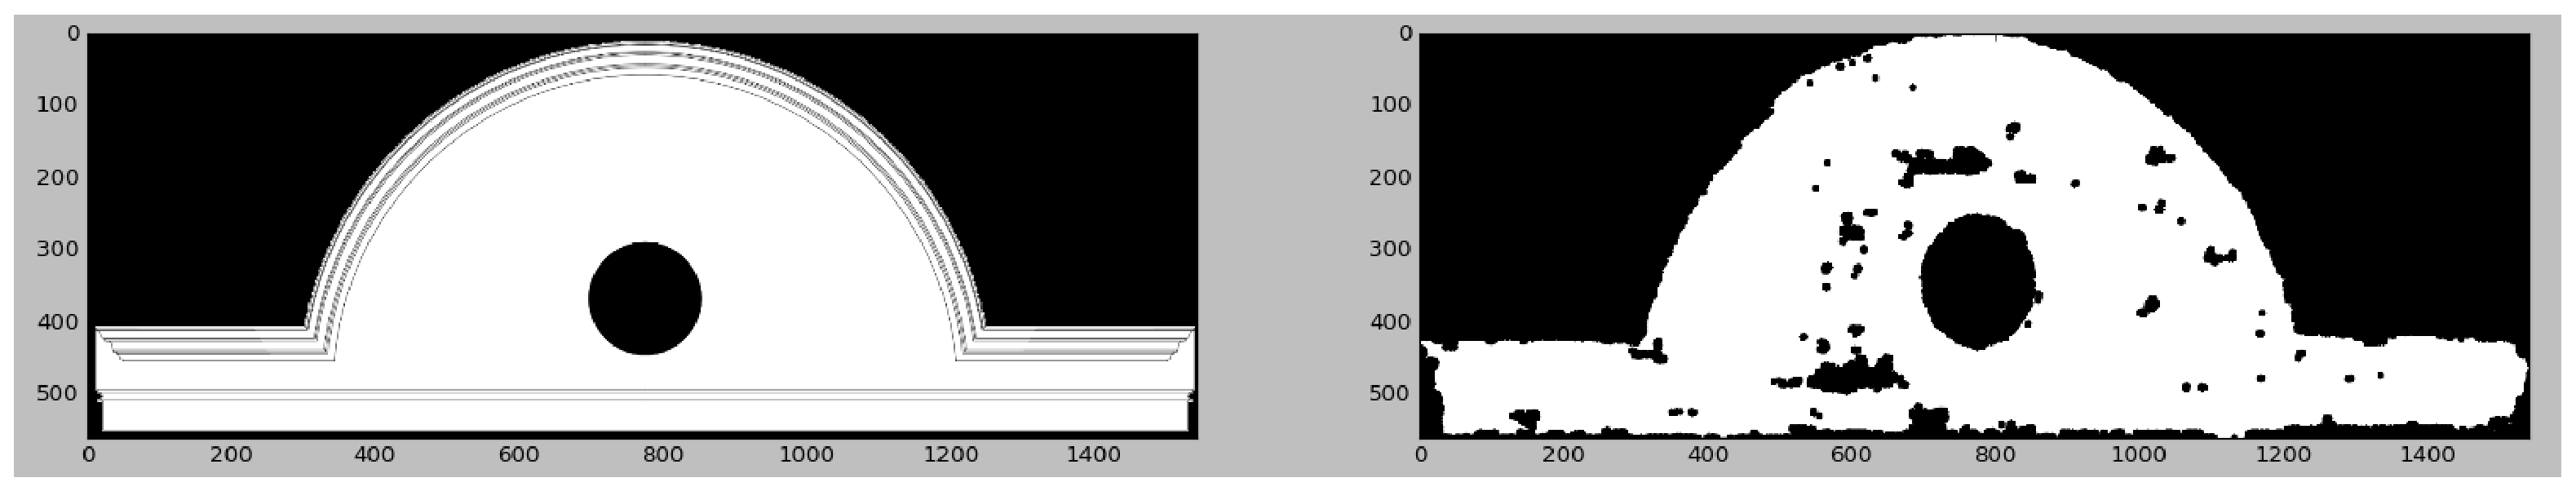
\includegraphics[width=8cm]{images/compare_clock}
        \end{center}
    \end{subfigure}
    \begin{subfigure}{1\linewidth}
        \begin{center}
            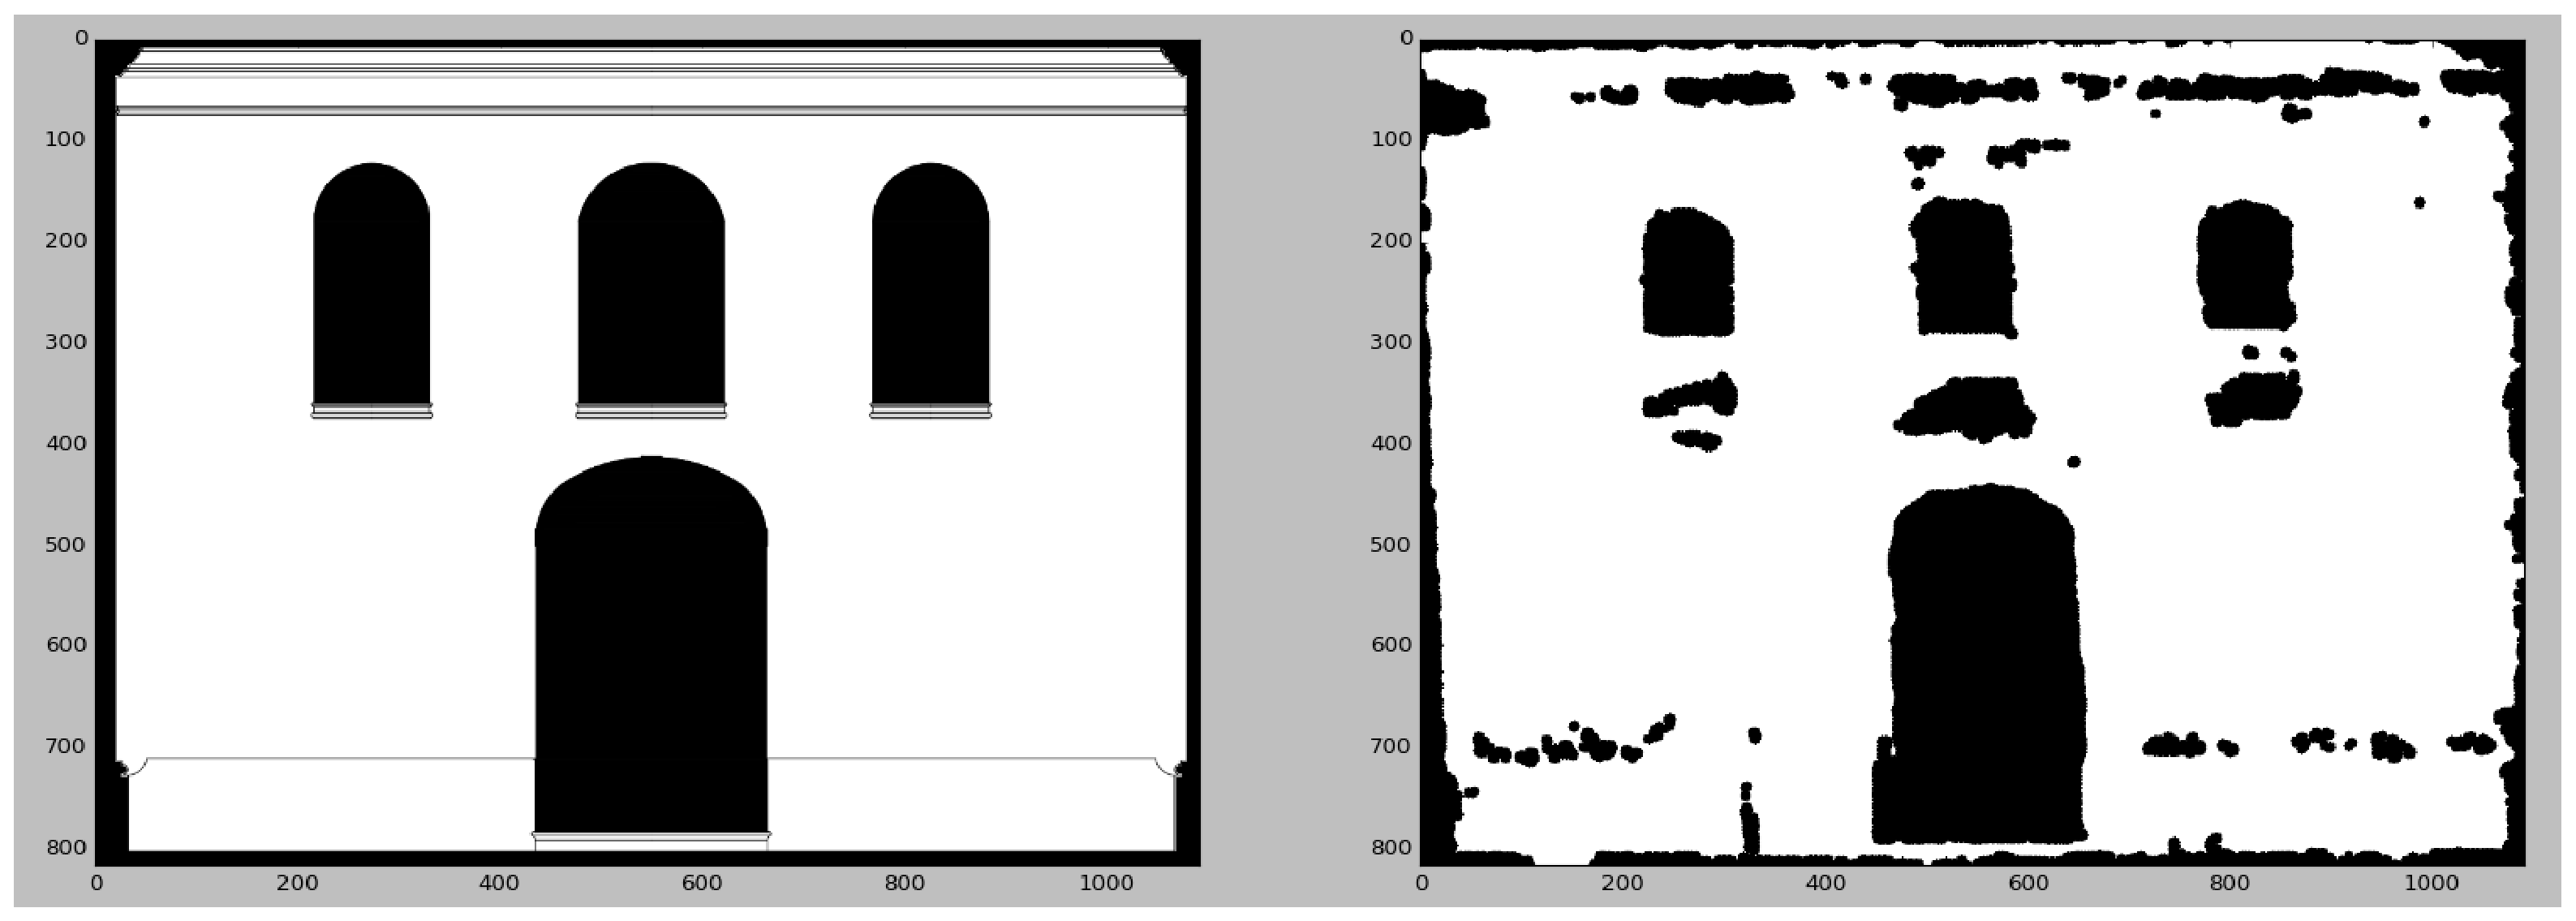
\includegraphics[width=8cm]{images/compare_wall}
        \end{center}
    \end{subfigure}
      \caption{Comparative among projections and project views. Source: author}
    \end{figure}
        
\end{frame}


\section{Conclusion}
\subsection{Partial Results}
\begin{frame}{Conclusion}
\framesubtitle{Partial Results}
    \justifying
    \begin{columns}
        \begin{column}{0.47\textwidth}
            \begin{figure}
              \vspace{-0.3cm}
              \centering
               {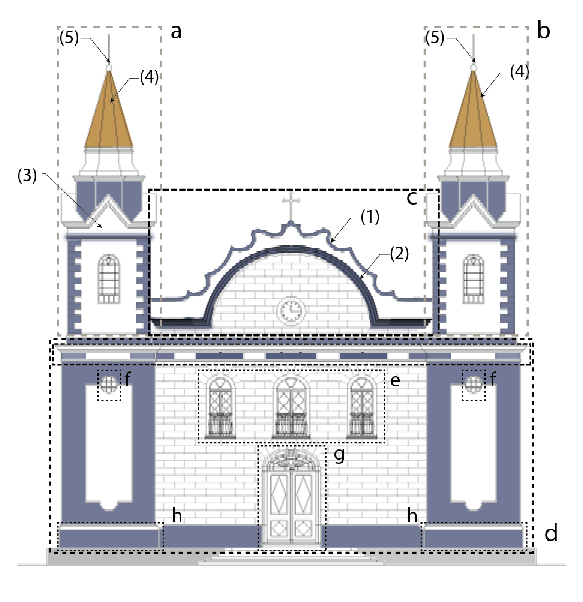
\epsfig{file = images/elementos, width = 3.5cm}}
             \end{figure}
        \end{column}
        \begin{column}{0.7\textwidth}
        \tiny\begin{itemize}
            \item[] a. Right Bell Tower;
            \item[] b. Left Bell Tower; 
            \item[] c. Double pediment with a clock on the tympanum. Straight cymatium (2) and scrolled pediment (1); 
            \item[] d. Frontispiece, with spare bell towers base (cornice highlighted in the figure made up of cymatium and friezes).
            \item[] g. Main door with lintel in segmental arch and door frame both in carved stone.
            \item[] h. Bell towers base;
            \end{itemize}
        \end{column}
    \end{columns}
    \vspace{-0.3cm}
    \tiny{
    \begin{table}
        \caption{Analysis of segmented regions compared to the as-designed model.}
        \centering
        \begin{center}
        \begin{tabular}{|c|c|c|c|}
              \hline
              COMPONENTS & PRECISION & RECALL &  ACCURACY\\
              \hline
              Frontispiece with voids of windows and doorways  &  87,73 & 93,37 & 85,76 \\
              \hline
              Tower base (right) & 94,63 & 86,56 & 84,79 \\
              \hline
              Tower base (left) & 94,34 & 94,68 & 90,89 \\
              \hline
              Right Bell Tower & 85,30 & 89,45 & 83,44 \\
              \hline
              Left Bell Tower  & 84,41 & 63,92 & 69,45 \\
              \hline
              Double pediment (tympanum and cymatium) & 55,68 & 39,29 & 82,32 \\
              \hline
              Scrolled pediment & 96,02 & 87,18 3 & 91,18 \\
              \hline
        \end{tabular}
        \end{center}

    \end{table}}
    
\end{frame}

\subsection{UAV and SfM popularization}
\begin{frame}
  \frametitle{Conclusion}
  \framesubtitle{UAV and SfM popularization}
  \justifying
    \begin{itemize}
        \item UAV popularization and SfM algorithms allow cultural heritage documenting and modelling
        \begin{itemize}[<+-| alert@+>]
            \item User-friendly
            \item Affordable
            \item But...
            \begin{itemize}
                \item Still needs formalization and reliability to eliminate experimental factor
            \end{itemize}
        \end{itemize}

        \item This work introduced a UAV image acquisition protocol able to produce strong representation for cultural heritage applications
        \vspace{-.4cm}
        \begin{itemize}[<+-| alert@+>]
            \item Ground stations proceedings
            \item SfM properties
        \end{itemize}
        \item Future analysis in method and application are necessary, especially with different heritage objects and SfM implementations.
    \end{itemize}
\end{frame}


\appendix

\begin{frame}[allowframebreaks]{References}
    \tiny
    \bibliography{bib}
    \bibliographystyle{plainnat}
\end{frame}

\begin{frame}[plain,c]
    \begin{center}
    \Huge Thank you!
    \end{center}
\end{frame}

\end{document}
